\documentclass{beamer}
\usepackage[utf8]{inputenc}
%\usepackage[latin1]{inputenc}
\usepackage{pifont}   %% tick and times symbols
\usepackage{amsmath}
\usepackage{amssymb}
%\usepackage{tabulary}
\usepackage{savesym}
\savesymbol{checkmark}
\usepackage{dingbat}
\usepackage{tabu}
\usepackage{listingsutf8}
%\usepackage{listings}
\usepackage{tikz} 
\usepackage{pgfplots}
\usepackage{graphicx}
\usepackage{color, colortbl}
%\usepgfplotslibrary{clickable}
\usetikzlibrary{shapes.callouts, decorations.text, decorations.pathreplacing, arrows.meta, automata, positioning, shapes.geometric}
\usepackage{hyperref}
%\usepackage{multimedia}
%\usepackage{media9}
\usepackage{multirow}
\usepackage{numprint} % provides rounding of float numbers 
\usepackage{pdfpages}
\usepackage{adjustbox}
\usepackage{pgf-umlsd}
\usepackage{algorithmic}
\usepackage[titlenotnumbered, linesnumbered]{algorithm2e}
\usepackage{booktabs} % For formal tables
\usetheme{uucs}
\setbeamercovered{invisible}

\usepackage{hyperref}
\hypersetup{
  colorlinks   = true, %Colours links instead of ugly boxes
  urlcolor     = uuyblue, %Colour for external hyperlinks
  linkcolor    = uuyred, %Colour of internal links
  citecolor    = uuygreen %Colour of citations
}


\newcommand{\Random}{\mathbb{R}}
\newcommand{\Genetic}{\mathbb{G}}
\newcommand{\RGenetic}{\mathbb{G}_{10}}

%%%%%%%%%%%%%%%%%%%%%%%%%%%%%%%%%%%%%%%%%%%%%%%%%%%%%%%%%%%%%
\definecolor{ltblue}{rgb}{0,0.4,0.4}
\definecolor{dkblue}{rgb}{0,0.1,0.6}
\definecolor{dkgreen}{rgb}{0,0.4,0}
\definecolor{dkviolet}{rgb}{0.3,0,0.5}
\definecolor{dkred}{rgb}{0.5,0,0}

\definecolor{lightgray}{rgb}{0.95, 0.95, 0.95}
\definecolor{darkgray}{rgb}{0.4, 0.4, 0.4}
%\definecolor{purple}{rgb}{0.65, 0.12, 0.82}
\definecolor{editorGray}{rgb}{0.95, 0.95, 0.95}
\definecolor{editorOcher}{rgb}{1, 0.5, 0} % #FF7F00 -> rgb(239, 169, 0)
\definecolor{editorGreen}{rgb}{0, 0.5, 0} % #007C00 -> rgb(0, 124, 0)
\definecolor{orange}{rgb}{1,0.45,0.13}		
\definecolor{olive}{rgb}{0.17,0.59,0.20}
\definecolor{brown}{rgb}{0.69,0.31,0.31}
\definecolor{purple}{rgb}{0.38,0.18,0.81}
\definecolor{lightblue}{rgb}{0.1,0.57,0.7}
\definecolor{lightred}{rgb}{1,0.4,0.5}
% CSS
\lstdefinelanguage{CSS}{
  keywords={color,background-image:,margin,padding,font,weight,display,position,top,left,right,bottom,list,style,border,size,white,space,min,width, transition:, transform:, transition-property, transition-duration, transition-timing-function},	
  sensitive=true,
  morecomment=[l]{//},
  morecomment=[s]{/*}{*/},
  morestring=[b]',
  morestring=[b]",
  alsoletter={:},
  alsodigit={-}
}

% JavaScript
\lstdefinelanguage{JavaScript}{
  morekeywords={typeof, new, true, false, catch, function, return, null, catch, switch, var, if, in, while, do, else, case, break, for},
  morecomment=[s]{/*}{*/},
  morecomment=[l]//,
  morestring=[b]",
  morestring=[b]'
}

\lstdefinelanguage{HTML5}{
  language=html,
  sensitive=true,	
  alsoletter={<>=-},	
  morecomment=[s]{<!-}{-->},
  morestring=[b]'
  tag=[s],
  otherkeywords={
  % General
  >,
  % Standard tags
	<!DOCTYPE,
  </html, <html, <head, <title, </title, <style, </style, <link, </head, <meta, />,
	% body
	</body, <body,
	% Divs
	</div, <div, </div>, 
	% Paragraphs
	</p, <p, </p>,
	% scripts
	</script, <script,
  % More tags...
  <canvas, /canvas>, <svg, <rect, <animateTransform, </rect>, </svg>, <video, <source, <iframe, </iframe>, </video>, <image, </image>, <header, </header, <article, </article
  },
  ndkeywords={
  % General
  =,
  % HTML attributes
  charset=, src=, id=, width=, height=, style=, type=, rel=, href=,
  % SVG attributes
  fill=, attributeName=, begin=, dur=, from=, to=, poster=, controls=, x=, y=, repeatCount=, xlink:href=,
  % properties
  margin:, padding:, background-image:, border:, top:, left:, position:, width:, height:, margin-top:, margin-bottom:, font-size:, line-height:,
	% CSS3 properties
  transform:, -moz-transform:, -webkit-transform:,
  animation:, -webkit-animation:,
  transition:,  transition-duration:, transition-property:, transition-timing-function:,
  }
}

\lstdefinelanguage{HTML5}{
  language=html,
  tagstyle=\color{blue},
  markfirstintag=true,
  sensitive=true,
  alsoletter={<>=-},	
  morecomment=[s]{<!--}{-->},
  % tag=[s],
  %% morestring=[b]'',
  morestring=[b]',
  ndkeywords={
    % General
    =,
    % HTML attributes
    id=, class= 
  }
}


\lstdefinestyle{htmlcssjs} {%
  % General design
  backgroundcolor=\color{editorGray},
  basicstyle={\scriptsize\ttfamily},   
  %frame=tb,
  % line-numbers
  xleftmargin={0.75cm},
  numbers=left,
  stepnumber=1,
  firstnumber=1,
  numberfirstline=true,	
  % Code design
  identifierstyle=\color{black},
  keywordstyle=\color{blue}\bfseries,
  ndkeywordstyle=\color{editorGreen}\bfseries,
  stringstyle=\color{editorOcher}\ttfamily,
  commentstyle=\color{brown}\ttfamily,
  % Code
  language=JavaScript,
  alsolanguage=HTML5,
  alsodigit={.:;},	
  tabsize=2,
  showtabs=false,
  showspaces=false,
  showstringspaces=false,
  extendedchars=true,
  breaklines=true,
  escapechar=|c
}
%%%%%%%%%%%%%%%%%%%%%%%%%%%%%%%%%%%%%%%%%%%%%%%%%%%%%%%%%%%%%


\title[ISSRE]{Test Data Generation for JavaScript Functions that Interact with the DOM}
\author[Elyasov et al.]{Alexander Elyasov, Wishnu Prasetya, \textbf{Jurriaan Hage}}
\institute[Universities Utrecht and Valencia]{
Utrecht University, The Netherlands \\ \texttt{alex.elyasov@gmail.com}
}
\date[ISSRE '18]{ISSRE '18, Memphis, TN, US}

\begin{document}
\frontmatter

\begin{frame}
  \titlepage
\end{frame}

\mainmatter

\begin{frame}
  \frametitle{Outline}
  %\transduration{10}
  \tableofcontents
\end{frame}


\section{Introduction}

\begin{frame}{StackOverflow Developer Survey}

  \footnotesize
  \begin{itemize}
    \item For the sixth year in a row, \emph{JavaScript} is the most commonly used programming language
    \item \emph{Node.js} and \emph{AngularJS} continue to be the most commonly used technologies, with \emph{React} also important to many developers
  \end{itemize}  

  \begin{columns}
    \column{.5\textwidth}{
      \centering
      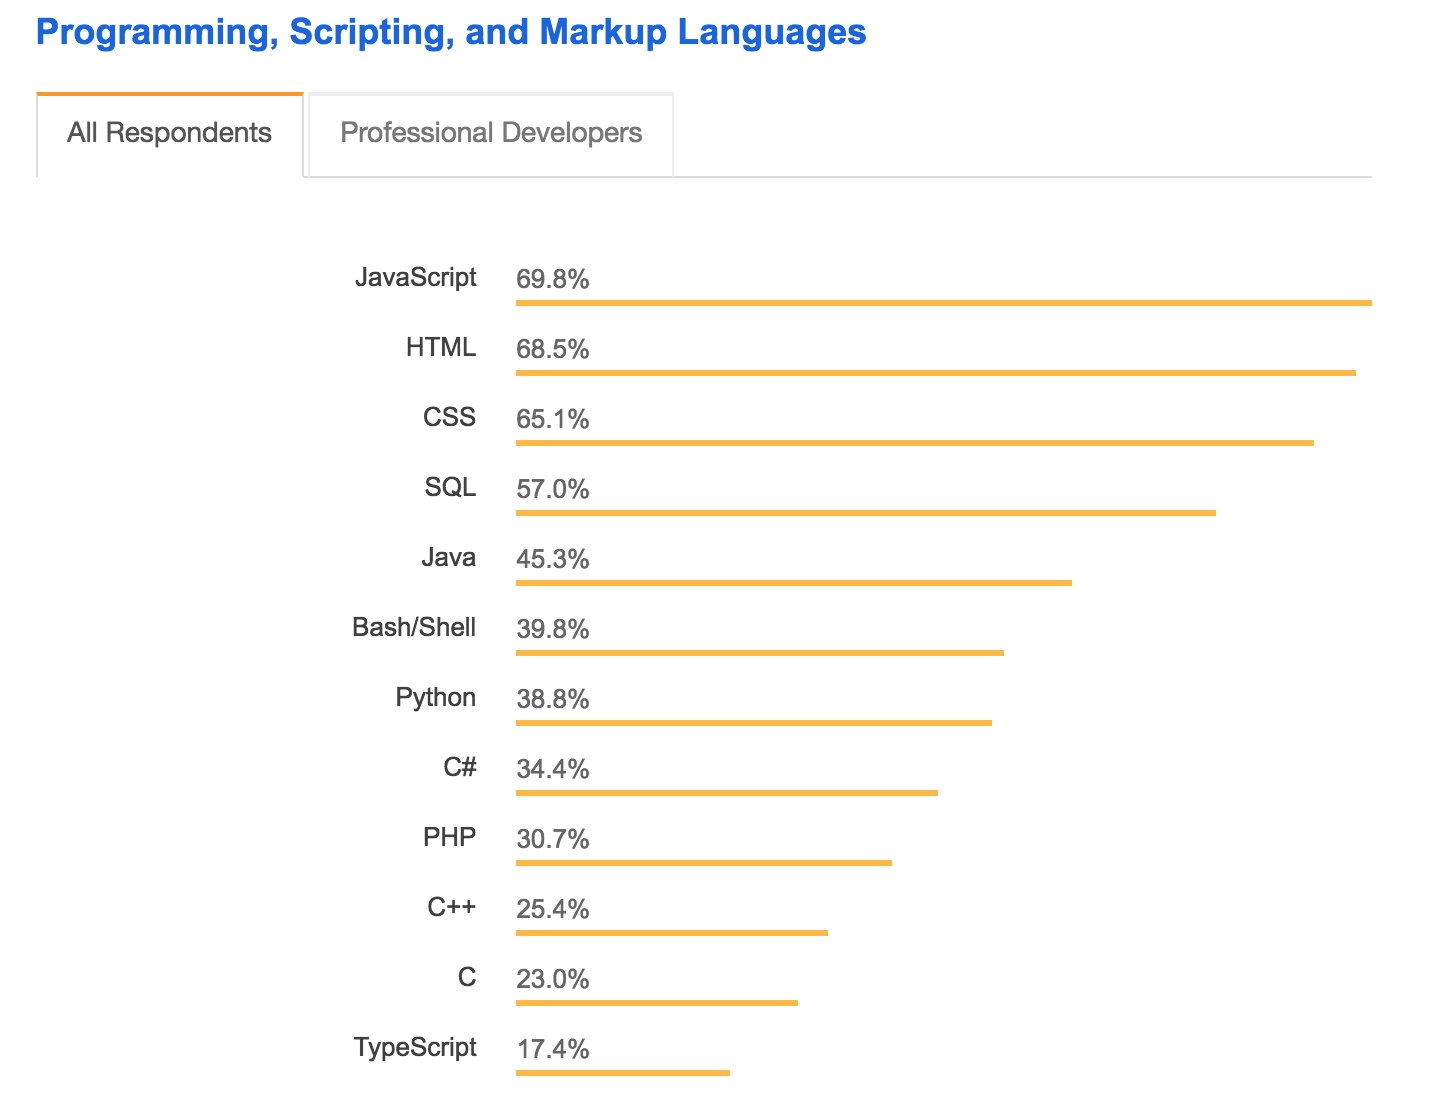
\includegraphics[scale=0.2]{JS_Popular.png}
    }
    
    \column{.5\textwidth}{
      \centering
      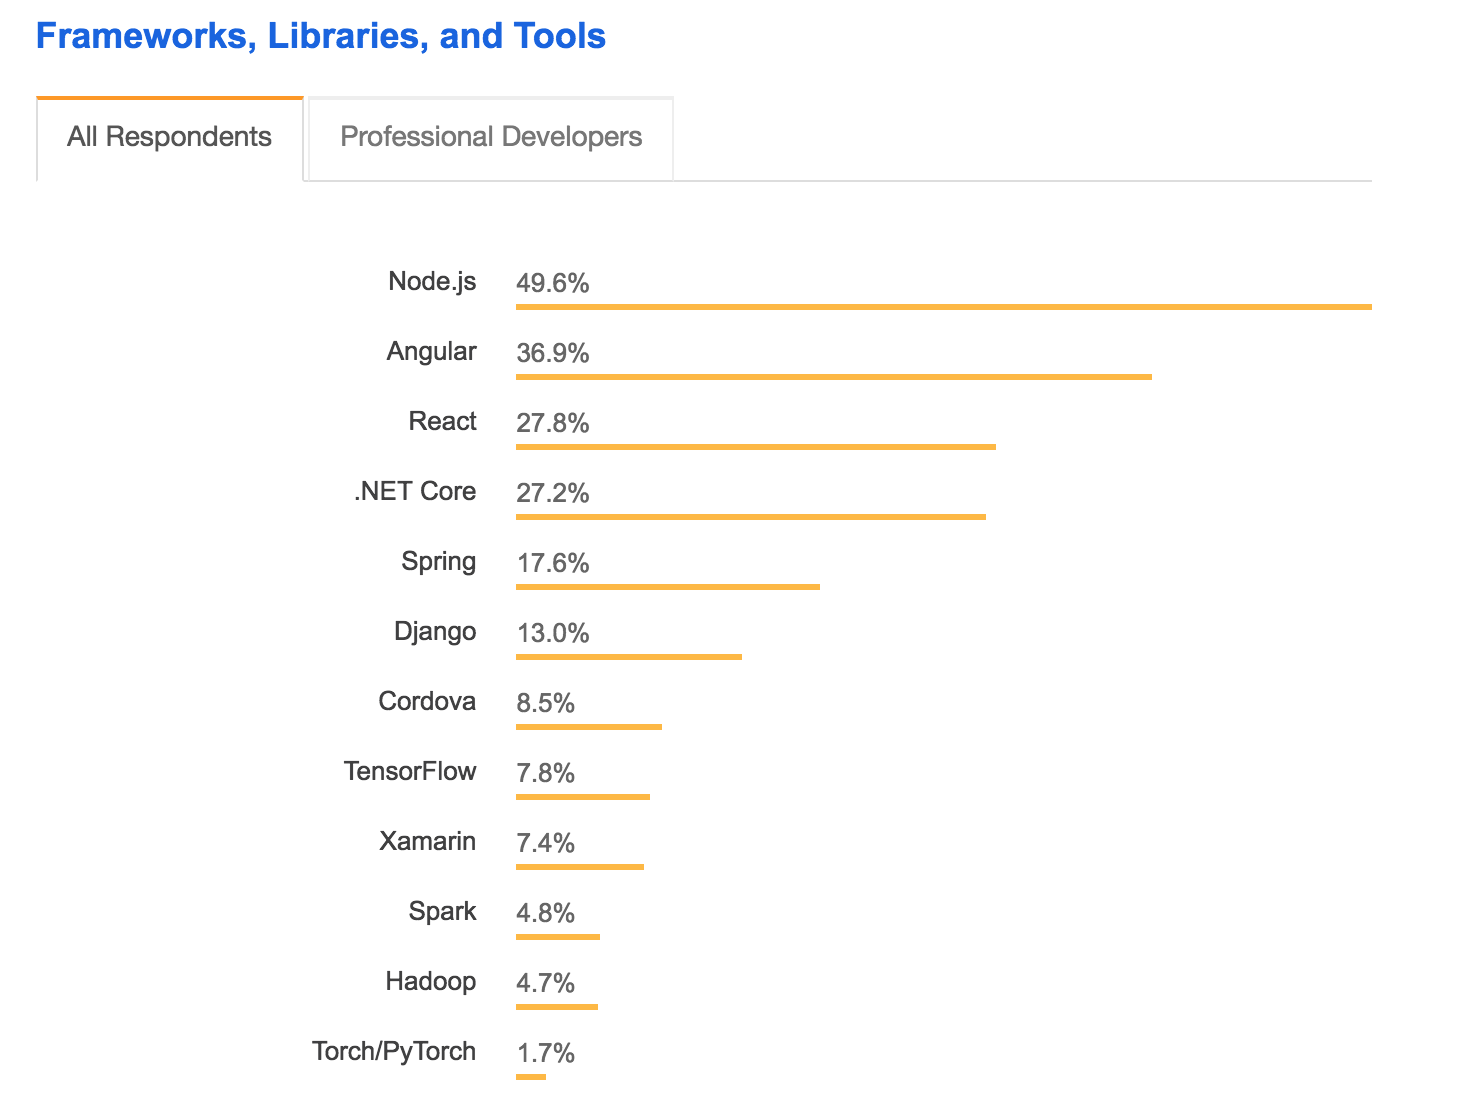
\includegraphics[scale=0.2]{NodeJS_Popular.png}
    }
  \end{columns}

  \begin{tikzpicture}[overlay]
    \draw[uuxred,line width=0.3mm] (0.2,3.3) rectangle (4.2,3.05);
    \draw[uuxred,line width=0.3mm] (6,3.3) rectangle (10,2.55);
  \end{tikzpicture}

\end{frame}

\begin{frame}{The State of JavaScript Testing}

  \begin{itemize}
    \item There exist numerous JS frameworks on the market:
      \begin{itemize}
        \item structure: Mocha, Jasmine
        \item assertions: Chai
        \item mocks and spies: Sinon
        \item coverage: Istanbul
        \item reporting: Karma
      \end{itemize}
   \item Developers report a relatively low happiness score with the state of testing tools
  \end{itemize}
  
  \centering{
    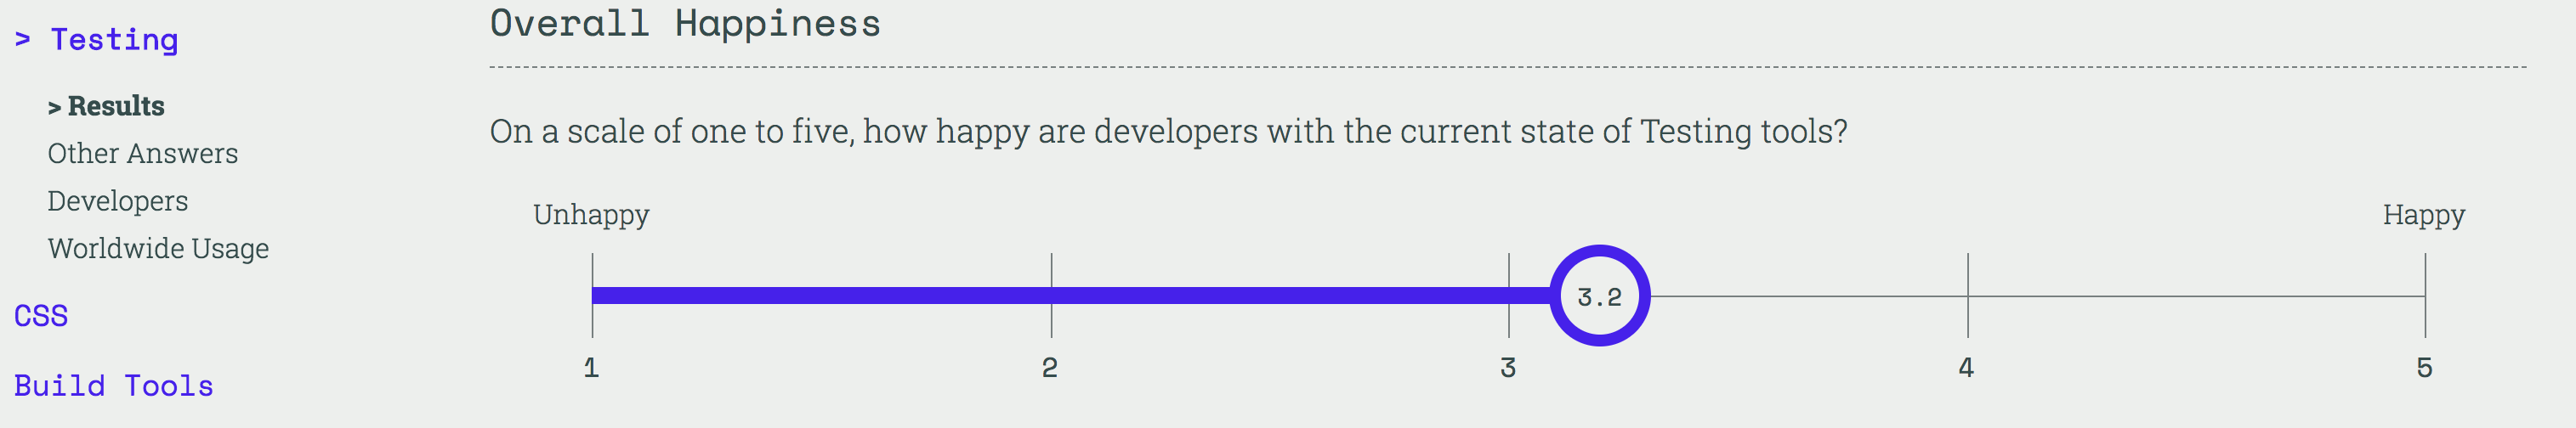
\includegraphics[width=10cm]{Unhappy_Devs.png}
  }
\end{frame}

\begin{frame}{Goal}
  \centering{
      
\includegraphics[width=7cm]{make.png}
  }
\end{frame}

\begin{frame}{Eureka!}
  \centering{
    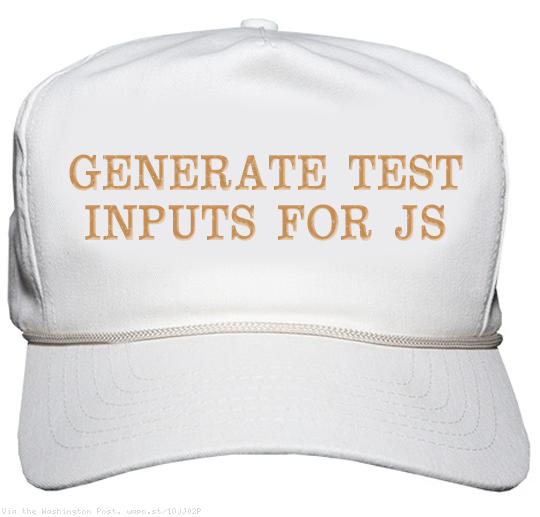
\includegraphics[width=7cm]{solution.png}
  }
\end{frame}

\begin{frame}{Test Input Generation}
  \begin{block}{Available techniques}
    \begin{itemize}
    \item concolic execution: \emph{Jalangi} and \emph{Confix}
    \item random generation: \emph{JSContest}
    \item static and dynamic analysis: \emph{Artemis}
    \item crawling: \emph{Crawljax}   
  \end{itemize}
  \end{block}
  
  \begin{block}{Input types}
    \begin{itemize}
      \item primitive types: numbers and strings
      \item collections: arrays
      \item objects
      \item DOM (focus of this paper)
      \item functions  
    \end{itemize}
  \end{block}
\end{frame}

\begin{frame}{Solution}

  \emph{JEDI}: \textbf{J}avascript \textbf{E}volutionary testing framework with \textbf{D}OM as an \textbf{I}nput

  \begin{block}{Contributions}
    \begin{itemize}
  \item implemented JEDI
  \item test generation algorithm
  \item  evaluation
    \end{itemize}
  \end{block}
\end{frame}

\section{Motivation Example}

\begin{frame}{Sudoku}
  \centering{
    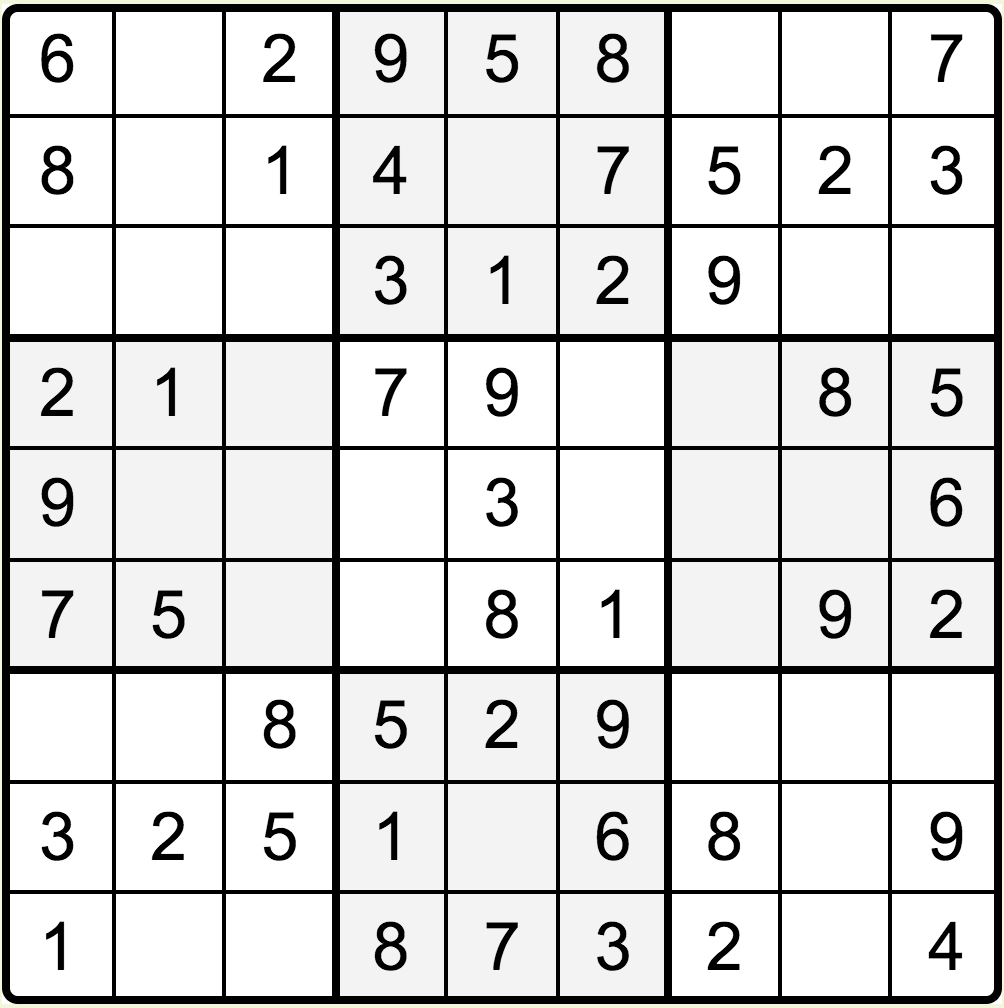
\includegraphics[width=7cm]{sudoku.png}
  }
\end{frame}  

\begin{frame}[fragile]{isGameFinished}

\begin{figure}
  \centering
  \begin{lstlisting}[style=htmlcssjs,language=JavaScript,basicstyle={\tiny\ttfamily}]
/*t dom */
function isGameFinished() {
  var obj = document.getElementById('sudoku'); 
  var subDivs = obj.getElementsByTagName('DIV'); 
  var allOk = true;
  for (var no = 0; no < subDivs.length; no++) { 
    if (subDivs[no].className.indexOf('square') >= 0 
        && !subDivs[no].style.backgroundColor) {
      var spans=subDivs[no].getElementsByTagName('SPAN');
      if (spans[0].innerHTML != spans[1].innerHTML) { 
       allOk = false; //target 
       break;
      }
    }
  } 
  return allOk;
}
  \end{lstlisting}
\end{figure}

\end{frame}

\begin{frame}[fragile]{DOM Tests}

\begin{figure}
  \begin{lstlisting}[style=htmlcssjs,language=HTML5,basicstyle={\tiny\ttfamily}]
<!-- T1: (5,5) -->            <!-- T2: (5,6), (7,15) -->
<html>                        <html>
 <body>                        <body>
  <div id='sudoku'>             <div id='sudoku'>
                                 <div></div>
  </div>                        </div>
 </body>                       </body>
</html>                       </html>

<!-- T3: (7,8), (10,14) -->   <!-- T4: (7,8), (10,11) -->
<html>                        <html>
 <body>                        <body>
  <div id='sudoku'>             <div id='sudoku'>
   <div class='square'>          <div class='square'>
    <span></span>                 <span></span>
    <span></span>                 <span>TEST</span>
   </div>                        </div>
  </div>                        </div>
 </body>                       </body>
</html>                       </html>
  \end{lstlisting}
\end{figure}  

\pause

  \begin{tikzpicture}[overlay]
    \draw[uuxred,line width=0.4mm] (4.5,4.1) rectangle (9,1);
  \end{tikzpicture}

\end{frame}

\begin{frame}[fragile]{T4 Explained}
\begin{adjustbox}{width=10cm}     \begin{lstlisting}[style=htmlcssjs,language=JavaScript,basicstyle={\tiny\ttfamily},mathescape=true]
/*t dom */
function isGameFinished() {
  var obj = document.getElementById('sudoku');   // $\mbox{\leftpointright}$ <div id='sudoku'>
  var subDivs = obj.getElementsByTagName('DIV'); // $\mbox{\leftpointright}$ <div class='square'>
  var allOk = true;
  for (var no = 0; no < subDivs.length; no++) { 
    if (subDivs[no].className.indexOf('square') >= 0  // $\mbox{\leftpointright}$ class='square'
        && !subDivs[no].style.backgroundColor) {
      var spans=subDivs[no].getElementsByTagName('SPAN');//$\mbox{\leftpointright}$ <span></span>
      // $\mbox{\leftpointright}$ <span>TEST</span>
      if (spans[0].innerHTML != spans[1].innerHTML) { 
       allOk = false; //target 
       break;
      }
    }
  } 
  return allOk;
}
  \end{lstlisting}
  \end{adjustbox}
\end{frame}

\section{Test Generation Framework}

\begin{frame}{Initialization Phase}
  \begin{figure}[!t]
  \centering
\tikzset{
  % add this style to all tikzpicture environments
  every picture/.append style={
    % enable scaling of nodes
    transform shape,
    % set scale factor
    scale=0.7
  }
}
  \begin{sequencediagram}[font=\footnotesize]

    \renewcommand\unitfactor{0.6}
    \newinst{user}{\textbf{User}}
    \newinst[1]{server}{\textbf{Server}}
    \newinst[4]{validator}{\textbf{Validator}}
    \newinst[1]{client}{\textbf{Client}}

    \begin{call}{user}{fun.js + config}{server}{\textbf{end}}
      \begin{call}{server}{Initialize(fun.js)}{server}{(cfg, branches, cinfo, ifun, sig)}
      \end{call}
      
      \begin{call}{server}{POST /init \{ifun, sig\}}{client}{status}
      \end{call}
      
      \begin{call}{server}{Select(branches)}{user}{$\text{branches}'$}
      \end{call}
      
    \end{call}
  \end{sequencediagram}
\end{figure}

\end{frame}

\begin{frame}{Algorithm I: Initialization Phase}
\begin{algorithm}[H]
  %% \algsetup{linenosize=\tiny} %% COMMENTED OUT IN PHD
  \footnotesize
  \DontPrintSemicolon
  \SetAlgoVlined
  \SetKwInOut{Input}{Input}
  \SetKwInOut{Output}{Output}
  \SetKwInOut{Require}{Require}
  \SetKwProg{Fn}{Function}{}{}
  \Input{JS file $fun.js$ with FUT and type annotation }
  \Output{Tuple $(cfg, branches, cinfo, ifun, sig)$}
  \Fn{$Initialize(fun.js)$}{

    $(ast, sig) \longleftarrow ParseFuncAndSig(fun.js)$\label{alg.init.parse.fun.sig}\;
    $cinfo \longleftarrow GetConstantInfo(ast)$\label{alg.init.collect.info}\;
    $nast \longleftarrow NormalizeAST(ast)$\label{alg.init.transform.ast}\;
    $ifun \longleftarrow Instrument(nast)$\label{alg.init.instr}\;
    $cfg \longleftarrow BuildCFG(nast)$\label{alg.init.build.cfg}\;
    $branches \longleftarrow GetBranches(cfg)$\label{alg.init.get.branches}\;
    \Return{$(cfg, branches, cinfo, ifun, sig)$}
    }
\end{algorithm}
\end{frame}

\begin{frame}{Supported Types}
\begin{block}{Type Annotation}
  /*t dom : bool : int : float : string : [int]  */
\end{block}
\begin{itemize}
\item primitive types: bool, int, float, sting
\item arrays
\item DOM
\item could be extended to objects
\end{itemize}
\end{frame}

\begin{frame}{Instrumentation}
\begin{itemize}
  \item \emph{trace} records the sequence of executed statements of the FUT
  \item \emph{branchDistance} contains the distance from the target branch
  \item \emph{loopMap} captures the upper bound for the number for-loop iterations  
\end{itemize}
\end{frame}

\begin{frame}{Genetic Phase}
\begin{figure}[!t]
  \centering
\tikzset{
  % add this style to all tikzpicture environments
  every picture/.append style={
    % enable scaling of nodes
    transform shape,
    % set scale factor
    scale=0.4
  }
}
  \begin{sequencediagram}[font=\normalsize]

    \renewcommand\unitfactor{0.55}
    \newinst{user}{\textbf{User}}
    \newinst[1]{server}{\textbf{Server}}
    \newinst[7]{validator}{\textbf{Validator}}
    \newinst[1]{client}{\textbf{Client}}

      \begin{sdblock}{\textbf{Genetic Loop}}{\small \hspace{8mm}$\text{branch} \in \text{branches}'$}
        \begin{sdblock}{\textbf{Random Loop}}{\small errors $>$ 0}
          \begin{call}{server}{pop = Random(cinfo, config)}{validator}{errors}
          \end{call}
          %\prelevel
        \end{sdblock}

        \begin{sdblock}{\textbf{Fitness Loop}}{\small (fitness $\neq$ 0) $\vee$ gen.limit}

          \begin{sdblock}{\textbf{Evaluation Loop}}{\small p $\in$ pop}
            \begin{call}{server}{POST /genetic \{p\}}{client}{response = ifun(p: sig)}
            \end{call}

            \begin{callself}{server}{Evaluate(branch, cfg, response)}{fitness}
            \end{callself}
            % \prelevel
          \end{sdblock}

          \begin{sdblock}{\textbf{Crossover Loop}}{\small errors $>$ 0}
            \begin{call}{server}{cross = Crossover(cinfo, pop)}{validator}{errors}
            \end{call}
            %\prelevel
          \end{sdblock}

          \begin{sdblock}{\textbf{Mutation Loop}}{\small errors $>$ 0}
            \begin{call}{server}{mut = Mutation(cinfo, pop)}{validator}{errors}
            \end{call}
            %\prelevel
          \end{sdblock}

          \begin{callself}{server}{pop = cross $\cup$ mut}{pop}
          \end{callself}
          %\prelevel
        \end{sdblock}
        \mess{server}{best fitness}{user}

      \end{sdblock}
  \end{sequencediagram}
\end{figure}
\end{frame}

\begin{frame}{HTML Generation}
  \begin{block}{Random}
    \begin{itemize}
      \item DSL for the generation of syntactically valid HTML documents composed of arbitrary \emph{tags} and \emph{attributes}
      \item multiple options for the parameterization: tree width and depth, tags frequency, etc.  
    \end{itemize} 
  \end{block}
  
  \begin{block}{GA operations}
    \begin{itemize}
      \item \emph{crossover} two HTML trees at a randomly chosen node
      \item HTML tree \emph{mutations}: \textit{NewTree}, \textit{DropTree} and \textit{ShuffleAttributes} (e.g. 'id' and 'class') 
    \end{itemize}
  \end{block}
 
  \end{frame}


\begin{frame}{Fitness Function (FF)}
\scriptsize
\begin{block}{FF for a node}
\begin{equation*}
F(n) = \textit{approach\_level} +
\begin{cases}
 1/2 * (\frac{\textit{branch\_distance}}{1 + \textit{branch\_distance}}) & \text{if no exception}\\
 1                                  & \text{otherwise}
\end{cases}
\end{equation*}
\begin{itemize}
  \item \emph{approach\_level} is the number of decision nodes between the target and the problem node (in JS every node can be exceptional)
  \item \emph{branch\_distance} measures the deviation explicitly in the problem node
\end{itemize}
\end{block}

\begin{block}{FF for a node sequence}
  \begin{equation*}
F^*(n_b, n_x) = (F(n_b), F(n_x))
\end{equation*}
\begin{itemize}
\item $n_b$ is a target branch node
\item $n_x$ is a terminal exit node
\item Can be generalized to: $F^*(n_1, n_2, \ldots, n_k) = (F(n_1), F(n_2), \ldots, F(n_k))$
\end{itemize}
\end{block}

\end{frame}

\begin{frame}{GA with Restart}
\begin{block}{Problem}
GA sometimes reaches a local minimum and stagnates due to flag variables, nested predicates, or unstructured control flow.
\end{block}
\begin{itemize}
  \item Common solution it to incorporate data dependency into the search, e.g. \emph{chaining approach}~\cite{ferguson1996chaining}
  \item Our approach is CFG-based because JS is a dynamic language which is hard to analyze for data dependency
  \item We suggest to restart GA with a new target when the fitness progress stops during a configured \emph{history window}
  \item The \emph{new target} consists of the original target prefixed by a dominating CFG node  
\end{itemize}
\end{frame}

\section{Empirical Evaluation}

\begin{frame}{Genetic Algorithm Configurations}

\begin{block}{Variations of Generation Algorithms}
\begin{itemize}
\item $\Random$  random
\item $\Genetic$  pure genetic
\item $\RGenetic$ genetic with restart
\end{itemize}

\end{block}

\begin{table}[!t]
  \footnotesize
  \centering
  \begin{tabular}{l|r|r|r}
    \toprule
    \textbf{Parameter Name} &$\Random$&$\Genetic$ &$\RGenetic$ \\
    \hline
    Population size                   & 50  & 50  & 50  \\
    Archive size                      & 1   & 25  & 25  \\
    Maximum number of generations     & 200 & 200 & 200 \\
    Crossover rate                    & 0   & 0.5 & 0.5 \\
    Mutation rate                     & 0   & 0.5 & 0.5 \\
    History window size               & -   & -   & 10  \\
    \bottomrule
  \end{tabular}
\end{table}
\end{frame}

\begin{frame}{Case Studies}
\setlength\tabcolsep{3pt}
\begin{table}[!t]
  %\resizebox{\textwidth}{!}{
    \tiny
    \centering
  \begin{tabular}{l|l|c|c|c|c|c|c|c|c}
    \toprule
    \textbf{case-study} & \textbf{function} & \textbf{loc} & \textbf{c} & \textbf{d} & \textbf{cc} & \textbf{dom} & \textbf{id} & \textbf{tag} & \textbf{class} \\
    \hline
    sudoku     & helpMe(int,int)    & 14 & 2 & 3 & 3 & + & + & + & - \\
    sudoku     & isGameFinished()    & 10 & 3 & 3 & 4 & + & + & + & + \\
    sudoku     & newGame()           & 9  & 1 & 2 & 2 & + & + & + & + \\
    sudoku     & revealAll()         & 8  & 0 & 2 & 1 & + & + & + & - \\
    %% sudoku     & - & showCell & (dom)          & 8  & 0 & 0 & 1 & + & + & + & - \\
    sudoku     & shuffleBoard(int,int)      & 23 & 2 & 3 & 3 & + & - & + & - \\
    %% sudoku     & - & switchLevel & (dom,bool)  & 10 & 1 & 2 & 2 & + & - & + & - \\
    \hline
    phormer    & toggleInfo(string)                                                     & 16 & 3 & 1 & 4 & + & + & - & - \\
    %% \multirow{2}{*}{phormer}    & \multirow{2}{*}{-} & \multirow{2}{*}{update} & (dom,int,[string],bool,[string],[string],bool,[string],[string],int) &    &   &   &   &   &   &   & \\
    %%            &   &        &                                                                      & 35 & 5 & 3 & 6 & + & + & - & - \\
    %% phormer    & - & updateIndic & (dom,bool)                                                      & 16 & 3 & 1 & 4 & + & + & - & - \\
    \hline
    %% hotel RS   & - & RequiredField & (dom,[string])  & 11 & 2 & 2 & 5 & + & + & - & - \\
    hotel RS   & isValidCard([int])           & 17 & 2 & 2 & 5 & - & - & - & - \\
    %% hotel RS   & - & isValidMasterCard & ([int])     & 5  & 4 & 1 & 7 & - & - & - & - \\
    hotel RS   & isValidVISA([int])           & 6  & 3 & 1 & 6 & - & - & - & - \\
    %% hotel RS   & - & validateNumber & (dom,string)   & 7  & 1 & 1 & 4 & + & + & - & - \\
    \hline
    %% apophis    & - & doRain & (dom,string,int,int,int,int,int,int)                                  & 10 & 3 & 2 & 4 & + & + & - & -\\
    %% apophis    & - & drawShields & (dom,[int])                                                      & 6  & 1 & 2 & 2 & + & + & - & - \\
    %% apophis    & - & fireMeteor & (int,[int],int,[int],[int],[int],int,int,[int],[int],int,int,int) & 15 & 3 & 2 & 4 & - & - & - & - \\
    %% apophis    & - & getReady & (dom,int,int,int,int,int,int)                                       & 16 & 2 & 2 & 3 & + & + & - & - \\
    apophis    & initShields([int],int,int)                                              & 6  & 0 & 1 & 1 & + & + & - & -\\
    \hline
    bingbong   & brickJiggler(int,int,[int],[int],[int],[int]) & 7  & 1  & 1 & 2  & + & + & - & - \\
    bingbong   & doPaddlePower(int,int)                            & 15 & 2  & 1 & 3  & + & + & - & - \\
    bingbong   & initBricks(int,[int],[int],[int],[int],int,[string])                         & 70 & 12 & 4 & 13 & + & + & - & - \\
    %% bingbong   & - & drawLevel & (dom,int,int,int,int)                        & 22 & 2  & 3 & 3  & + & + & - & - \\
    %% bingbong   & - & goPing & (dom,int,int,int)                               & 12 & 2  & 2 & 3  & + & + & - & - \\
    \hline
    burncanvas & do\_draw(int,int,int,int,int,int,int)                 & 40 & 12 & 2 & 14 & - & - & - & - \\
    %% \hline
    %% cs-in-js   & - & luhn-algorithm & (string,bool)                          & 20 & 3 & 2 & 6 & -  & -  & - & - \\
    %% cs-in-js   & - & quicksort-partition & ([int],int,int)                   & 21 & 1 & 1 & 3 & -  & -  & - & - \\
    \hline
    mathjs     & prob\_gamma(float)                                   & 57 & 8  & 2 & 16 & - & - & - & - \\
    \bottomrule
  \end{tabular}
%}
\end{table}

\begin{itemize}
\item if $\text{CC} < 10$ then the function is \emph{easy to test} else \emph{difficult} 
\end{itemize}

\end{frame}

\begin{frame}{Research Questions}
\begin{description}
\item[RQ1] What is the branch coverage?
\item[RQ2] What is the coverage time per branch?
\item[RQ3] Are the results statistically significant?
\item[RQ4] What is the branch coverage of \emph{Confix}?
\end{description}
\end{frame}

\section{Results}

\begin{frame}{RQ1: What is the branch coverage?}
  
  \begin{table}
    \footnotesize
    \caption{Branch coverage (\%)}
    \begin{tabular}{c|ccc}
      \toprule
      \textbf{TYPE}  & $\Random$  & $\Genetic$ & $\RGenetic$\\
        \midrule
      \textbf{simple (23)}    & 79 & 97 & 100  \\
      \textbf{difficult (33)} & 58 & 94 & 100 \\
      \midrule
      \textbf{global (56)}    & 63 & 95 & 100 \\
      \bottomrule
    \end{tabular}
  \end{table}

  \begin{block}{}
    Across all subjects, the $\RGenetic$ algorithm achieved 100\% branch coverage, with $\Genetic$ in the second place with 95\% coverage, and, finally, $\Random$ with  63\% coverage.
  \end{block}
 
\end{frame}

\begin{frame}{RQ1: Branch Coverage Progress}
  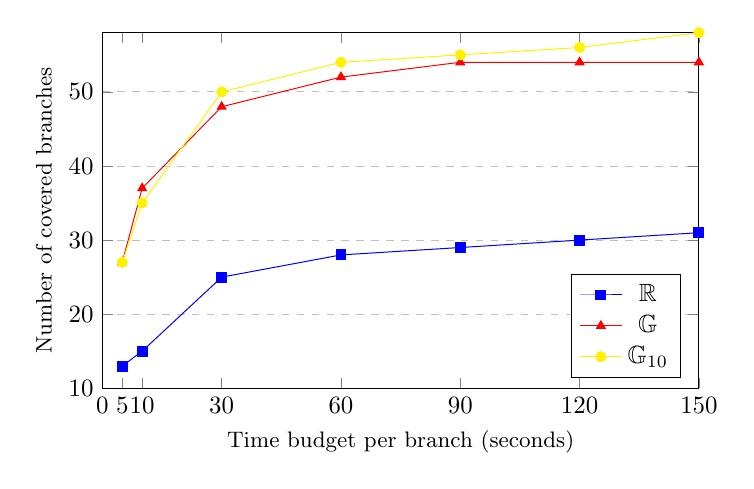
\begin{tikzpicture}[scale=0.9]
    \begin{axis}[
        xlabel={Time budget per branch (seconds)},
        ylabel={Number of covered branches},
        width=10cm,height=6.6cm,
        xmin=0, xmax=150,
        ymin=10, ymax=58,
        xtick={0,5,10,30,60,90,120,150,180},
        ytick={0,10,20,30,40,50},
        legend pos=south east,
        ymajorgrids=true,
        % xmajorgrids=true,
        grid style=dashed,
        label style={font=\small}
      ]

      \addplot[
        color=blue,
        mark=square*,
      ] coordinates {
        (5,13) (10,15) (30,25) (60,28) (90,29) (120,30) (150,31)
      };
      \addplot[
        color=red,
        mark=triangle*,
      ]  coordinates {
        (5,27) (10,37) (30,48) (60,52) (90,54) (120,54) (150,54)
      };
      \addplot[
        color=yellow,
        mark=*,
      ]   coordinates {
        (5,27) (10,35) (30,50) (60,54) (90,55) (120,56) (150,58)
      };
      \legend{$\Random$,$\Genetic$,$\RGenetic$}

    \end{axis}
  \end{tikzpicture}
 

  \begin{block}{}
    $\Genetic$ could be more suitable for rapid testing during development, whereas $\RGenetic$ for integration
  \end{block}
  
\end{frame}

\begin{frame}{RQ2: What is the coverage time per branch?}
  
  \begin{table}
    \footnotesize
    \centering
    \caption{Average execution time per brunch (sec.)}
    \begin{tabular}{c|ccc}
      \toprule
      \textbf{TYPE} & $\Random$ & $\Genetic$ & $\RGenetic$ \\
      \midrule
      \textbf{simple (23)}    & 37  & 9  & 7   \\
      \textbf{difficult (33)} & 112 & 56 & 25  \\
      \midrule
      \textbf{global (56)}    & 88  & 39 & 19  \\
      \bottomrule
    \end{tabular}
  \end{table}

\begin{block}{}
  $\RGenetic$ outperformed both $\Genetic$ and $\Random$ with an average execution time per branch of 19, 39 and 88 seconds, respectively.
\end{block}

\begin{block}{}
    On average, one algorithm iteration took one second for $\Random$ and $\RGenetic$, $\Genetic$ performed somewhat worse at 1.4 seconds.
\end{block}

\end{frame}

\begin{frame}{RQ3: Are the results statistically significant?}
  \footnotesize
  \begin{table}
     \scriptsize
     \centering
     %\caption{Significance and effect size}
     \begin{tabular}{c|p{3mm}p{3mm}p{3mm}|p{3mm}p{3mm}p{3mm}|p{3mm}p{3mm}p{3mm}}
      \toprule
      \multirow{2}{*}{\textbf{TYPE}} & \multicolumn{3}{c|}{$\Random / \Genetic$} & \multicolumn{3}{c|}{$\Random / \RGenetic$} & \multicolumn{3}{c}{$\Genetic / \RGenetic$} \\
      \cline{2-10}
      %\hline
                              & L  & M  & S  & L  & M  & S  & L & M & S \\
      \midrule
      \textbf{simple (23)}    & 11 & 12 & 13 & 11 & 13 & 13 & 1 & 1 & 1 \\
      \textbf{difficult (33)} & 22 & 24 & 26 & 22 & 23 & 26 & 2 & 2 & 4 \\
      \midrule
      \textbf{global (56)}    & 33 & 36 & 39 & 33 & 36 & 39 & 3 & 3 & 5 \\
      \bottomrule
    \end{tabular}
\end{table}

\begin{itemize}
  \item Use the non-parametric Mann-Whitney U-test and the Vargha-Delaney $\hat{A}_{12}$ statistics for measuring statistical significance ($\alpha=0.05$) and effect size~\cite{arcuri2011practical}
    \item L - large  (0.71), M - medium (0.64), S - small (0.56)
\end{itemize}

\begin{block}{}
    Both $\Genetic$ and $\RGenetic$ largely outperform $\Random$ in 50\% cases generally across the board and 67\% on the difficult functions.
\end{block}
\end{frame}

\begin{frame}{RQ4: What is the branch coverage of Confix?}
\begin{table}
  \scriptsize
  \setlength\tabcolsep{2pt}
    \begin{tabular}{c|l|c|c|c|c|c}
      \toprule
      \textbf{case-study} & \textbf{function} & \textbf{\#BR} & \textbf{\#C (weak)} & \textbf{\#C (strong)} & \textbf{\#tests} & \textbf{time (sec.)} \\
      \hline
      sudoku & helpMe          & 5  & 4 (80\%)  & 4 (80\%)  & 2 & 5 \\
      sudoku & isGameFinished  & 5  & 2 (40\%)  & 2 (40\%)  & 2 & 5 \\
      sudoku & newGame         & 3  & 3 (100\%) & 3 (100\%) & 4 & 6 \\
      sudoku & revealAll       & 2  & 2 (100\%) & 0 (0\%)   & 6 & 11 \\
      sudoku & shuffleBoard    & 7  & 5 (71\%)  & 0 (0\%)   & 2 & 5  \\
      \hline
      phormer & toogleInfo     & 4  & 2 (50\%)  & 2 (50\%)  & 3 & 5 \\
      \hline
      apophis & initShields    & 1  & 0 (0\%)   & 0 (0\%)   & 1 & 6 \\
      \hline
      bingbong & brickJiggler  & 2  & 0 (0\%)   & 0 (0\%)   & 1  & 3 \\
      bingbong & doPaddlePower & 4  & 2 (50\%)  & 2 (50\%)  & 1  & 4 \\
      bingbong & initBricks    & 18 & 3 (17\%)  & 0 (0\%) & 1  & 3 \\
      \bottomrule
    \end{tabular}
\end{table}
\begin{block}{}
The choice between a concolic and search-based approach is a trade-off between a labour-intensive modelling and execution time, respectively, where both can reinforce each other.
\end{block}

\end{frame}


\begin{frame}{Threats to Validity}
\begin{itemize}
  \item \emph{construct validity}: measured only branch coverage and execution time
    \begin{itemize}
      \item it doesn't indicate fault finding capability
      \item use only ``natural'' oracles such as exception
      \item ignore test case size
    \end{itemize}    
  \item \emph{internal validity}: choice of the initial GA configuration 
  \item \emph{conclusion validity}: stochastic nature of the experiment
  \item \emph{external validity}: limited set of experimental subjects 
\end{itemize}
\end{frame}

\section{Future Work and Conclusions}

\begin{frame}{Future Work}
\begin{itemize}
  \item the whole test suite generation based on multi-objective optimization to balance coverage and test suite size~\cite{panichella2017lips}
    \item mutation driven test generation~\cite{fraser2012mutation}; should allow us to evaluate fault finding capability
    \item combine search-based with concolic test generation for JavaScript, e.g. integrate \emph{Jalangi}~\cite{sen2013jalangi} and~\emph{Confix}~\cite{amin:ase15}
      \item conduct large evaluation of \emph{JEDI}; it requires the extension of arbitrary input objects and functional arguments~\cite{claessen2011quickcheck, selakovic2018test}
\end{itemize}
\end{frame}

\begin{frame}{Conclusions}
  \begin{itemize}
    \item introduced a novel search-based JS unit testing framework, called \emph{JEDI}, which is able to generate arbitrary DOM inputs
     \item presented a test generation algorithm ---``genetic with restart''; it is capable of escaping plateaus by concretizing the search target
     \item conduced an empirical validation followed by the significance study, which has confirmed the effectiveness and efficiency of our framework in branch coverage testing 
 
  \end{itemize}
\end{frame}


\begin{frame}[t,allowframebreaks]{References}
\tiny
\bibliographystyle{alpha}
\bibliography{issre2018}
\end{frame}

\begin{frame}{The End}
\begin{center}
  \vspace{-2em}
  \emph{Thanks for attention!}\\
  \vspace{1em}
  \emph{Questions?}\\
  \vspace{2em}
  %% \href{http://www.facebook.com/FITTESTproject}{
\includegraphics[height=1.5cm,keepaspectratio]{pict/logo/facebook}}~%
  %% \href{https://plus.google.com/112865571538811672642}{
\includegraphics[height=1.5cm,keepaspectratio]{pict/logo/gplus}}~%
  \href{https://github.com/aelyasov/JSDomTest}{
\includegraphics[height=1.5cm,keepaspectratio]{pict/logo/git}}%
\end{center}
\end{frame}

\end{document} 
